\chapter{Primitives de mouvement}
\label{chap:primitive}

\epigraph{Vous n'avez qu'à marcher de vertus en vertus.}{Jean
  Racine\\\emph{Britannicus}}
\clearpage

\section{Problématique}

\lettrine[lines=2, lraise=0.1, nindent=0em, slope=-.5em]%
{L}{e} chapitre précédent a introduit la possibilité d'asservir une
trajectoire de marche sur un robot humanoïde. Cependant, les tâches
accomplies par les robots humanoïdes ne se limitent pas à la
locomotion et il est intéressant de se demander s'il est possible de
combiner aux tâches de navigation d'autres tâches asservies par les
données capteurs afin de réaliser des comportements complexes. De
manière indirecte, la question qui se pose ici est celle de la limite
à placer entre d'une part raisonnement numérique et d'autre part
raisonnement logique. Ce problème récurrent de la robotique et pour
lequel il n'existe pas, de consensus au sein de la communauté trouve
ici une solution élégante. En effet, un contrôleur fondé sur le
paradigme de la pile de tâches\index{pile de tâches} ne se limite pas
à une description d'objectifs ou de contraintes robotiques dans des
espaces plus naturels que l'espace des configurations ou l'espace
cartésien, il ouvre surtout la voie à des mécanismes de supervision
décidant à quel moment insérer telle ou telle tâche à un niveau de
priorité donné. La pile de tâches réalise donc la jonction entre d'une
part, le monde du calcul numérique puisque la finalité du système est
de calculer la commande du système et d'autre part le monde de la
logique dans lequel les utilisateurs humains souhaitent exprimer leur
\emph{desiderata} au système robotique: va jusqu'à la cuisine,
apporte-moi la bouteille, ouvre la porte, etc. Il est clair que ce
type d'ordre nécessite la résolution d'abstractions et que la logique
mathématique semble être un moyen particulièrement adapté pour y
parvenir. Ces mécanismes de décision de haut niveau sont appelés
``superviseurs'' et ont pour objectif d'instancier et d'orchestrer
tous les composants d'une architecture robotique. Dans le cadre de
notre architecture, il faut donc pouvoir instancier des piles de
tâches à partir d'une description de haut niveau des ordres passés au
robot. Ce chapitre propose un langage de description des tâches
permettant de faire le lien entre représentation logique et
représentation numérique.


Nous allons commencer par détailler l'état de l'Art et en particulier
les autres travaux ayant trait aux architectures robotiques haut
niveau et à l'ordonnancement de tâches ainsi que plus généralement aux
applications robotiques complexes. Dans un second temps, le langage de
description sera décrit et quelques scénarii types seront
démontrés. Enfin, nous nous concentrerons sur les problèmes
d'asservissement posés par les robots humanoïdes avant de conclure.


\section{État de l'Art}


La perception et l'exécution de tâches asservies en robotique
représentent deux domaines particulièrement actifs. Un livre de
référence sur la localisation robotique et le SLAM\index{Simultaneous
  Localization and Mapping (SLAM)}, le domaine lié à la cartographie
et localisation simultanée en robotique est \cite{05thrun}. Les
travaux de navigation en robotique humanoïdes sont plus rares. On peut
citer les travaux de James Kuffner, Joel Chestnutt, Koichi Nishiwaki
-- \begin{CJK*}{UTF8}{min}正西脇 光一\end{CJK*} --
  \cite{05michel.humanoids,05ozawa.smc,03chestnutt.humanoids,02nishiwaki.rsj}
  de l'Université de Freiburg en Allemagne \cite{10osswald.icra}. Dans
  le domaine la vision pour les humanoïdes, l'utilisation de
  l'asservissement visuel a été tenté \cite{10dune.iros} ainsi que des
  techniques de SLAM telles que
  \cite{06stasse.iros,09kwak.humanoids}. Une introduction à
  l'asservissement visuel\index{asservissement visuel} est
  \cite{06chaumette.ram,07chaumette.ram}. La possibilité d'utiliser un
  robot humanoïde pour la modélisation automatique d'objets 3D a
  également été envisagée par \cite{09foisotte.icra,08stasse.ras}. Une
  approche fondée sur la replanification à partir de données vision
  sur HRP-2\index{HRP-2} a également été publiée dans
  \cite{11dang.humanoids}.


\section{Description d'un mouvement robotique complexe}


Décrire le comportement d'une pile de tâches\index{pile de tâches}
revient à décrire deux éléments primordiaux: d'une part les tâches
exprimées dans le solveur et de l'autre les différents changements
d'état de la pile au cours du mouvement. Concernant les
tâches\index{tâche}, il s'agit ici de représenter des fonctions
mathématiques génériques ne présentant pas de point commun permettant
une représentation générique de ces dernières. Par exemple si l'on se
limitait aux fonctions linéaires $\mathbf{A}(t) \mathbf{x} +
\mathbf{b}(t)$, encoder la matrice $\mathbf{A}$ et le vecteur
$\mathbf{b}$ serait envisageable pour un ensemble discret de valeurs
$t$ données. Le cas évoqué est trop contraint pour notre problème et
les modélisations informatiques développées dans le
\autoref{chap:chap1} n'aide pas: elles ont pour but de venir fournir
un modèle pour l'expression d'une fonction mathématique sous la forme
d'un algorithme et non pas sous la forme d'une donnée structurée
pouvant facilement être encodée. Le choix a donc été fait de définir
un ensemble de tâches permettant de réaliser un certain nombre
d'actions intéressantes. Rien n'empêche alors cet ensemble de
``primitives'' d'être étendu au cours du temps mais il nécessite
l'extension du modèle de description défini ici.


La seconde partie est la représentation des changements d'état. Un
changement d'état du solveur survient quand une tâche est: ajoutée,
supprimée ou bien encore quand sa priorité est modifiée. De manière
générale les transitions peuvent être soit temporelles -- avance de 5
mètres puis saisis la poignée de la porte --, soit logique -- si tu es
à moins de 10 cm de la position finale, arrête-toi --. Pour comprendre
la stratégie choisie, il faut garder à l'esprit que pour réaliser un
scénario complexe certains comportements seront intégrés dans la
boucle temps réel tandis que d'autres -- typiquement les informations
capteurs -- seront traitées à l'extérieur. Les deux catégories
d'événements, temporelle ou logique, ne mettent pas en jeu les mêmes
mécanismes. Les événements temporels sont décidés à l'avance et
doivent être exécutés avec une grande précision pour assurer un
comportement correct du système tandis que les événements logiques
sont le résultat d'un mécanisme de décision externe.

De ce fait, la stratégie adoptée a été de permettre la représentation
de transitions temporelles dans le modèle de description uniquement
tandis que l'on considère que les transitions événementielles, de fait
plus lentes et difficiles à encoder, sont gérées à l'extérieur du
contrôleur par un logiciel décisionnel ayant la possibilité de
regénérer le mouvement s'il devient invalide suite à la réception
d'une nouvelle donnée capteur. De nombreux logiciels adaptés à cette
tâche ont été développés tel que SMACH\footnote{Site web officiel:
  \url{http://www.ros.org/wiki/smach}}.


\subsection{Primitive de mouvement}
\index{primitive de mouvement}

La première tâche a été de définir des primitives de mouvement de
haut niveau. Les primitives proposées sont:
\begin{enumerate}
\item La locomotion\index{locomotion}: mouvement synchronisé des deux
  jambes et du centre de masse du robot pour réaliser un déplacement
  tout en assurant sa stabilité.
\item La manipulation\index{manipulation} et le contact: mouvement
  réalisant le placement d'une partie spécifiée du robot à un
  emplacement donné dans l'espace euclidien. La tâche peut contraindre
  la position et/ou la rotation du corps à positionner.
\item Regard ou asservissement visuel\index{asservissement visuel}: le
  robot doit maintenir un point dans son champ de vision.
\end{enumerate}


\subsection{Primitive de locomotion}

Une tâche de locomotion est définie initialement comme une série de
points de contact à réaliser pour atteindre une position
finale. Chacun des points de contact\index{point de contact} étant
annoté par l'effecteur devant réaliser le contact à cet endroit. À
partir de ces informations, une trajectoire des effecteurs réalisant
les appuis est déduite ainsi que du centre de masse pour préserver
l'équilibre dynamique du système. Afin de pouvoir utiliser les
techniques décrites dans le \autoref{chap:suivi}, nous nous limiterons
à la marche sur un sol plat utilisant le pied gauche et le pied droit
du robot. Le calcul de la trajectoire des effecteurs et du centre de
masse est encore un problème ouvert à l'heure actuelle. Les modèles
simples peuvent être embarqués dans les contrôleurs au prix de
nombreuses simplifications détaillées dans le chapitre précédent
tandis que les modèles les plus compliqués nécessitent une résolution
hors du contrôleur rendant le comportement du système non réactif. Le
chapitre précédent a proposé une stratégie pour fusionner les
avantages des deux approches. Nous considérons ici la totalité de
l'approche développée au cours du chapitre précédent comme une
implémentation d'une primitive de locomotion. En particulier, l'erreur
de positionnement du robot est considérée comme une entrée de la
primitive de mouvement.


\subsubsection{Tâche d'alignement de deux repères}

Cette primitive de mouvement repose principalement sur la définition
d'une tâche où le solveur doit positionner un corps du robot à un
endroit précis à la fois en rotation et en translation. C'est cette
tâche qui va permettre de faire suivre la trajectoire des pieds
notamment.

\begin{figure}
  \begin{center}
    \begin{equation}
      \left (
      \begin{array}{cccc}
        \cline{1-4}
        \multicolumn{1}{|c}{R_{11}} & R_{12} & R_{13} & \multicolumn{1}{|c|}{t_x} \\
        \multicolumn{1}{|c}{R_{21}} & R_{22} & R_{23} & \multicolumn{1}{|c|}{t_y} \\
        \multicolumn{1}{|c}{R_{31}} & R_{32} & R_{33} & \multicolumn{1}{|c|}{t_z} \\
        \cline{1-4}
        0 & 0 & 0 & 1
      \end{array}
      \right )
    \end{equation}
  \end{center}
  \caption{Structure d'une matrice homogène représentant un élément de
    $\text{SE}(3)$: les coefficients $R_{i,j}$, $(i,j) \in \{1,
    \dotsc, 3\}$ forment la matrice de rotation associé à la
    transformation et $\{t_x, t_y, t_z\}$ le vecteur de
    translation. Une matrice de rotation ayant elle-même une forme
    contrainte: elle doit être une matrice orthogonale de déterminant
    1. \label{fig:matrixhomo}}
\end{figure}


Soit $\mathbf{M}, \mathbf{M}^{*} \in \text{SE}(3)^2$
respectivement la position actuelle du corps du robot et la position
de référence à atteindre. On peut alors définir l'erreur de cette
tâche comme:

\begin{equation}\label{eq:featurepoint6d}
  \mathbf{e} = \mathbf{M} (\mathbf{M}^{*})^{-1}
\end{equation}

On remarquera que dans (\autoref{eq:featurepoint6d}), $\mathbf{e}$ est
un élément de $\text{SE}(3)$. Les éléments de $\text{SE}(3)$ peuvent
s'exprimer de nombreuses façons différentes: matrice homogène -- 16
paramètres --, translation et quaternion -- 7 paramètres
--\index{quaternion}, vecteur de rotation -- 6 paramètres --
\index{vecteur (de rotation)}, etc. Il faut garder à l'esprit qu'une
paramétrisation minimale de $\text{SE}(3)$ nécessite six
paramètres. De fait, tout représentation utilisant un espace de
dimension supérieure vient avec un ensemble de contraintes à respecter
car tous les éléments de cet espace de dimension supérieur ne peuvent
faire parti de $\text{SE}(3)$. Par exemple, une matrice homogène a une
structure bien particulière tel qu'illustré sur la
\autoref{fig:matrixhomo}. Quant aux quaternions, seuls les quaternions
unitaires définissent une bijection avec $\text{SO}(3)$, l'espace des
rotations dans l'espace 3d.

De fait, les représentations non minimales ne constituent pas une
solution acceptable pour représenter notre erreur, car elles
provoquent l'insertion de contraintes supplémentaires inutiles dans le
problème d'optimisation. Il faut donc choisir pour représenter
$\mathbf{e}$ une représentation minimale, dans notre cas par une
translation et une rotation autour d'un axe.

En effet, toute rotation peut être représentée par trois paramètres
\mbox{$\mathbf{\theta} = (\alpha, \beta, \gamma) \in \mathbb{R}^3$}. Le
vecteur $(\alpha, \beta, \gamma)$ normalisé représentant l'axe autour
duquel la rotation s'effectue et la norme du vecteur
$|\mathbf{\theta}|$ la quantité de rotation réalisée autour de cet
axe, voir \autoref{fig:utheta}.

\begin{figure}
  \begin{center}
    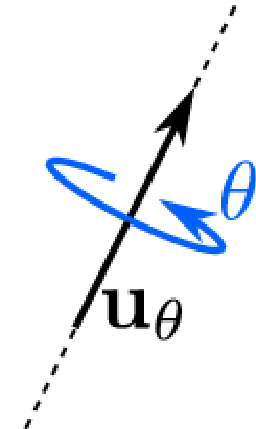
\includegraphics[width=.1\linewidth]{src/chap3-primitive-mouvement/utheta.pdf}
  \end{center}
  \caption{Représentation d'une rotation par un axe de rotation $u$ et
    une quantité de rotation $\theta$. Une représentation minimale à
    trois paramètres est possible en posant: $\theta = |u|$. \label{fig:utheta}}
\end{figure}


Cette représentation est minimale, car la translation est représentée
par trois paramètres et la rotation par trois paramètres:

\begin{equation}
  \mathbf{e} = \left(
  \begin{array}{c}
    t_x\\
    t_y\\
    t_z\\
    \theta_x\\
    \theta_y\\
    \theta_z
  \end{array}
  \right)
\end{equation}

En considérant les trois premiers éléments du vecteur d'erreur ou bien
les trois derniers, on peut restreindre la tâche à positionner le corps
respectivement en translation ou en rotation uniquement.


\subsubsection{Tâche de position du centre de masse}


Le second type de tâche nécessaire pour définir la primitive de
locomotion est la tâche de positionnement du centre de masse.

Cette tâche nécessite la connaissance du poids de tous les corps du
robot $m_i$ où $i \in \mathcal{B}$. $\mathcal{B}$ l'ensemble des corps
du robot. Le centre de masse\index{centre de masse} du robot est alors
défini comme le barycentre des centres de masse de chaque corps:

\begin{equation}
  \mathbf{x} = \frac{1}{\sum_{i \in \mathcal{B}} m_i} \sum_{i \in \mathcal{B}} m_i \mathbf{x}_i
\end{equation}

$\mathbf{x}$ représentation la position du centre de masse du robot et
$\mathbf{x}_i$ la position du centre de masse du corps $i$.

L'erreur de positionnement du centre de masse est alors simplement:

\begin{equation}
  \mathbf{e} = \mathbf{x} - \mathbf{x}^{*}
\end{equation}

La définition de l'erreur ne posant pas de difficulté ici car
$\mathbf{x}$ est un élément de $\mathbb{R}^3$.


\subsubsection{Définition de la primitive de locomotion}

Une tâche de locomotion est par nature critique: un mauvais suivi de
la trajectoire de référence du centre de masse ou bien encore de la
trajectoire des pieds aboutit à une perte de l'équilibre du robot. De
ce fait, établir une priorité entre ces tâches n'a pas de sens. On
préférera donc exprimer ces trois tâches -- pied gauche, pied droit et
centre de masse -- de la façon suivante:

\begin{equation}
  \mathbf{e} = \mathbf{e}_{\text{pied gauche}} + \mathbf{e}_{\text{pied droit}} + \mathbf{e}_{\text{centre de masse}}
\end{equation}

Les équations formulées dans cette section peuvent enfin être
paramétrées par le temps courant $t$ afin de permettre une
modification de la valeur de référence notée $\mathbf{M}^*$ ou
$\mathbf{x}^*$ selon les cas et permettre le suivi d'une trajectoire
plutôt que l'atteinte d'une référence constante.


Comme décrit dans le chapitre précédent, l'erreur des tâches décroît
exponentiellement -- dans le cas où la référence reste constante
--. Un suivi suffisamment précis de la trajectoire est alors
réalisable en augmentant suffisamment $\lambda$ le gain associé à la
tâche. Dans la mesure où l'erreur initiale de cette tâche est nulle --
le mouvement commence à la position actuelle du robot -- et varie de
manière continue, la tâche ne génère pas de grandes vitesses
articulaires malgré le gain important.


\subsubsection{Primitive de manipulation}


La primitive de manipulation est une instance directe de la tâche
d'alignement de repères présentée dans la section précédente. Elle
est utilisée pour placer la main à un endroit donné afin de saisir un
objet. Le déplacement d'un bras du robot ne mettant pas en jeu
l'équilibre du robot tant qu'elle se déplace peu rapidement et sans
perturber la tâche de suivi du centre de masse, on peut simplement
corriger l'erreur de positionnement de la main avec une interpolation
linéaire pour amener la main à la position désirée.


\subsubsection{Primitive de regard}


La dernière primitive introduite ici concerne l'asservissement de la
trajectoire du robot afin de préserver des amers dans une zone où
elles sont détectables par les capteurs du robot. Sur le robot HRP-2,
seul des caméras sont à la disposition des utilisateurs et leur
placement dans la tête permet naturellement de définir une tâche de
``regard'' où l'utilisateur souhaite garder un point au centre de
l'image captée par une caméra du robot.

Soit \mbox{$M = (X, Y, Z) \in \mathbb{R}^3$} un point 3d dont les
coordonnées sont définies par rapport à la position de la caméra du
robot et \mbox{$m = (x, y) \in \mathbb{R}^2$} sa projection sur le
plan image de la caméra\index{géométrie projective}. On a alors la
relation suivante:

\begin{equation}
  \mathbf{m} = \left(
  \begin{array}{c}
    x\\
    y
  \end{array}
  \right) = \left(
  \begin{array}{c}
    X / Z\\
    Y / Z
  \end{array}
  \right)
\end{equation}


Une fois de plus l'erreur se définit par la soustraction usuelle:

\begin{equation}
  \mathbf{e} = \mathbf{m} - \mathbf{m}^*
\end{equation}

\begin{figure}
  \begin{center}
    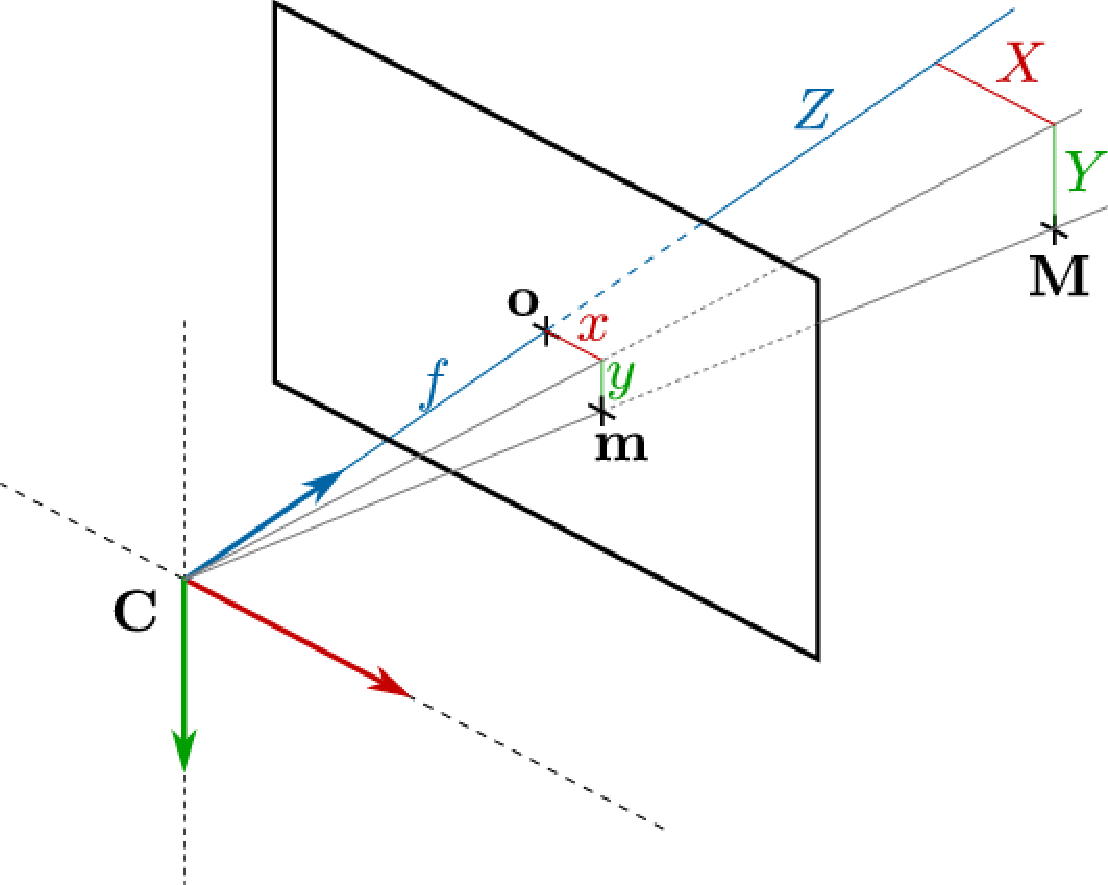
\includegraphics[width=.95\linewidth]{src/chap3-primitive-mouvement/cameraProj.pdf}
  \end{center}
  \caption{Projection du point 3D $M = (X, Y, Z)$ sur le plan image
    d'une caméra idéale. Les coordonées du point projeté sont ici $m =
    (x, y)$. $f$ est la distance focale de la caméra et $o$ le centre
    optique, deux paramètres intrinsèques de la caméra.}
\end{figure}




\subsection{Langage de description}

Le langage de description adopté est le YAML -- Yet Another Markup
Language -- \citep{yaml}\index{Yet Another Markup Language (YAML)}. Le
fichier est divisé en trois parties:
\begin{description}
\item[En-tête] fournissant les méta-informations sur le mouvement,
  notamment sa durée en secondes.
\item[Primitives de mouvement] définissant quelles primitives sont
  jouées et sur quel intervalle, ainsi que la configuration de chaque
  primitive.
\item[Primitives d'asservissement] définissant comment l'erreur de
  positionnement du robot est estimée au fil du temps.
\end{description}


\subsubsection{Primitive de locomotion}
\index{primitive!de locomotion}

Une primitive de locomotion est définie par un ensemble de points de
contacts définis sur la forme d'une pile de pas.

\begin{description}
\item[Intervalle] Date de début et de fin de la primitive de mouvement.
\item[Empreinte de pas] Liste des pas à effectuer. Les pas sont
  considérés comme des éléments de $\text{SE}(2)$ dans la mesure où
  l'algorithme de génération de pas fait l'hypothèse d'un sol plan.
\end{description}

Lors du chargement du plan, la génération des trajectoires de pieds et
de centre de masse initiales est réalisée hors ligne de manière
asynchrone. Tant que le calcul n'est pas terminé, il n'est pas
possible de lancer le mouvement.


\subsubsection{Primitive de manipulation}
\index{primitive!de manipulation}

Une primitive de manipulation est définie par un corps et une position
6d de référence. L'objectif est de faire coïncider le corps avec la
position 6d de référence. Cette tâche peut ne considérer que la
rotation ou la translation.

\begin{description}
\item[Intervalle] Date de début et de fin de la primitive de manipulation.
\item[Corps à considérer] Nom du corps à considérer. Des noms
  génériques ont été définis tels que: cheville gauche, cheville
  droite, poignet gauche, poignet droit, tête, torse et bassin.
\item[Consigne] La position de référence vers laquelle le corps doit
  être amené. Il peut être de trois types. Soit statique, le corps
  doit maintenir sa position initiale, soit fixe dans ce cas le corps
  doit atteindre un point prédéterminé de l'espace, soit dynamique
  dans ce cas le corps doit suivre un point mobile.
\end{description}


\subsubsection{Primitive de regard}
\index{primitive!de regard}

La primitive de regard définit comment le robot peut maintenir son
regard vers un point 3d, éventuellement mobile.

\begin{description}
\item[Intervalle] Date de début et de fin de la primitive de manipulation.
\item[Caméra à considérer] Nom de la caméra utilisée. En pratique, la
  caméra est définie comme un corps ``virtuel'' du robot et l'on peut
  donc potentiellement aligner n'importe quelle partie du corps du
  robot vers un point donné.
\item[Consigne] La position de référence vers lequel le corps doit
  pointer. Il peut être de deux types. Soit fixe, dans ce cas le corps
  doit pointer vers un point prédéterminé de l'espace, soit dynamique
  et dans ce cas le corps doit pointer vers un point mobile.
\end{description}


\subsubsection{Asservissement des primitives sur les données capteur}


Une fois la séquence de mouvement définie, il faut encore pouvoir
fermer la boucle sur les données capteur. Dans le cadre d'un mouvement
complexe, une stratégie intéressante est de pouvoir s'asservir
successivement sur plusieurs amers afin de planifier \emph{a priori}
quelle est la ou les amers les plus pertinentes à différents instants.


Soit $\mathcal{L}$ un système de localisation. Un système de
localisation est défini comme une fonction qui à tout instant fournit
une pose estimée d'un corps de référence du robot, dans notre cas le
bassin. On a donc:

\begin{equation}
  \begin{array}{ccc}
    \mathcal{L} : & \mathbb{R} \rightarrow & \text{SE}(2)\\
      & t \mapsto & \mathcal{L}(t)
  \end{array}
\end{equation}

Au cours du mouvement, $n$ systèmes de localisation fournissent une
estimation de la pose du robot. Une fois de plus, cette pose est
théoriquement dans l'espace 3D $\text{SE}(3)$, mais les contraintes
physiques font que seuls trois degrés de liberté doivent être
réellement estimés: $(x, y, \theta) \in \text{SE}(2)$. Ces trois
degrés correspondent à la position 2D de la projection du bassin sur
le sol. De ce fait, l'interpolation de $n$ poses 2D et la moyenne des
poses à la normalisation de l'angle $\theta$ prêt.


On associe à chaque système de localisation une fonction de poids
déterminant l'influence relative des systèmes de localisation dans
l'estimation finale de la pose:

\begin{equation}
  \begin{array}{ccc}
    m_i : & \mathbb{R} \rightarrow & \mathbb{R}\\
      & t \mapsto & m_i(t)
  \end{array}
\end{equation}

La fusion des données pour l'estimation de la pose est donc le
barycentre des poses 2d:

\begin{equation}
  \mathbf{\hat{x}}(t) = \frac{1}{\sum_{i \in n} m_i} \sum_{i \in n} m_i \mathcal{L}_i(t)
\end{equation}

En pratique, chaque système de localisation est représenté de la façon suivante:
\begin{description}
\item[Poids] en fonction du temps. Il peut soit être constant, soit
  varier dynamiquement.
\item[Erreur] de positionnement en fonction du temps. Elle est fournie
  par un système de localisation externe.
\end{description}


\section{Scénarii de mouvements}


Nous allons voir ici plusieurs exemples de mouvements décrits en
utilisant le langage de description introduit dans la section
précédente. L'objectif est à la fois de démontrer la généricité de
l'approche par plusieurs scénarii différents ainsi que sa mise en
\oe uvre pratique.


\subsection{Locomotion simple}

Le premier scénario consiste en le déplacement du robot le long d'une
pile de pas prédéterminée pendant 20 secondes. La description
complète du plan est fournie par la \autoref{fig:plan_locomotion_simple}.

\begin{figure}
  \begin{center}
\begin{verbatim}
duration: 20 # durée complète du mouvement (secondes)

# Éléments de mouvement
motion:
  # Primitive de locomotion
  - walk:
      interval: [0, 20] # Date de début et de fin de la primitive

      # Pile de pas
      footsteps:
      - {x: 0.15, y: -0.19, theta: 0.}
      - {x: 0.15, y: +0.19, theta: 0.1}
      # etc.
\end{verbatim}
  \end{center}
  \caption{Plan de mouvement pour une séquence de marche non asservie.\label{fig:plan_locomotion_simple}}
\end{figure}

La marche est effectuée en boucle ouverte et l'erreur d'exécution
n'est pas compensée. Chaque pas est exprimé relativement au pas
précédent. Le corps effectuant chaque contact peut être déduit de la
séquence d'empreinte de pas: si la translation en $y$ du premier pas
dispose d'un signe négatif, le premier pas est effectué avec le pied
droit, sinon avec le pied gauche. L'alternance pied gauche/pied droit
à chaque pas est ensuite implicite.


Il n'y a pas, à ce niveau de vérification de la faisabilité des
pas. C'est le rôle du planificateur de s'assurer préalablement à la
génération du plan de mouvement que la séquence est réalisable.

\begin{figure}
  \begin{center}
    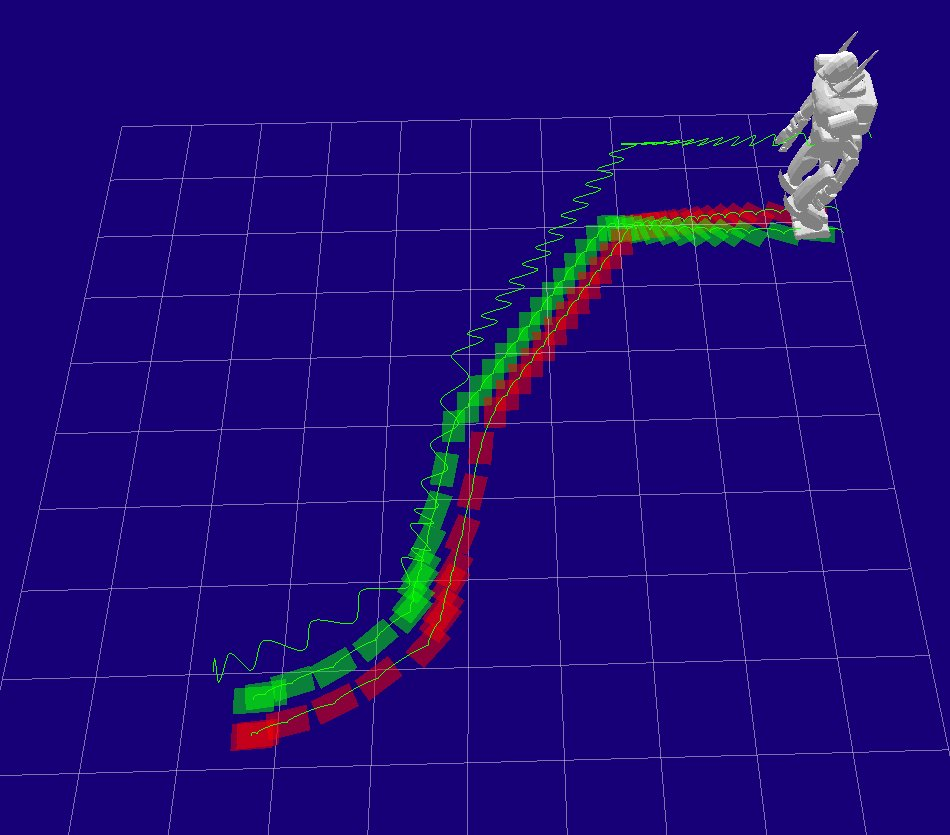
\includegraphics[width=.95\linewidth]{src/chap3-primitive-mouvement/footsteps1.jpg}
  \end{center}
  \caption{Exemple de pile de pas à partir de laquelle une primitive
    de locomotion peut être calculée.}
\end{figure}


\FloatBarrier

\subsection{Locomotion asservie}

On peut se demander désormais comment asservir la locomotion en
utilisant un composant de localisation. La
\autoref{fig:plan_locomotion_asservie} fournit une version alternative
du plan précédent ajoutant la correction de pas introduite dans le
\autoref{chap:suivi}.

\begin{figure}
  \begin{center}
\begin{verbatim}
duration: 20 # durée complète du mouvement (secondes)

# correction maximum autorisée sur un pas (x, y en mètre, theta en radians)
maximum-correction-per-step: {x: 0.02, y: 0.02, theta: 0.05}

# Éléments de mouvement
motion:
  # Primitive de locomotion
  - walk:
      interval: [0, 20] # Date de début et de fin de la primitive

      # Pile de pas
      footsteps:
      - {x: 0.15, y: -0.19, theta: 0.}
      - {x: 0.15, y: +0.19, theta: 0.1}
      # etc.

# Asservissement des tâches
servoing:
  # Asservissement via le système de capture de mouvements.
  - mocap:
      weight: 1.
      tracked-body: left-ankle
      perceived-body: left-foot
\end{verbatim}
  \end{center}
  \caption{Plan de mouvement pour une séquence de marche asservie sur
    un système de localisation -- ici un système de capture de
    mouvement --.\label{fig:plan_locomotion_asservie}}
\end{figure}

La seconde partie du plan décrit que l'erreur de positionnement
provient d'un unique système de localisation. Dans ce cas, un système
de capture de mouvement. Plusieurs systèmes de localisation ont été
testés pour fournir une estimation de la position du robot au cours du
mouvement:

\begin{description}
\item[Capture de mouvement] Ce système permet une localisation
  quasi-parfaite permettant de s'abstraire de la plupart des problèmes
  de perception.
\item[Suivi d'un objet] Un système réalisant le suivi d'un objet dans
  l'image captée par une caméra du robot et reconstituant sa position
  3d peut également être utilisé. Dans ce cas, on suppose l'objet fixe
  dans le monde et on en déduit la position du robot.
\item[SLAM] Les techniques de SLAM -- Simultaneous Localization and
  Mapping -- permettent de cartographier l'environnement tout en
  fournissant une estimation de la position actuelle du robot. La
  carte enregistrée permet d'assurer une localisation sans dérive
  quelque soit la longueur du mouvement à condition de pouvoir
  identifier des amers précédemment détectées régulièrement le long
  du mouvement.
\end{description}

\begin{figure}
  \begin{center}
\begin{verbatim}
duration: 20 # durée complète du mouvement (secondes)

# correction maximum autorisée sur un pas (x, y en mètre, theta en radians)
maximum-correction-per-step: {x: 0.02, y: 0.02, theta: 0.05}

environment:
  - object:
      name: table
      planned:
        position:
          x: 1.75
          y: 0.3
          z: -0.3
          rx: 0.
          ry: 0.
          rz: 2.

# Éléments de mouvement
motion:
  # Primitive de locomotion
  - walk:
      interval: [0, 20] # Date de début et de fin de la primitive

      # Pile de pas
      footsteps:
      - {x: 0.15, y: -0.19, theta: 0.}
      - {x: 0.15, y: +0.19, theta: 0.1}
      # etc.

# Asservissement des tâches
servoing:
  # Asservissement via le système de capture de mouvements.
  - visp:
      weight: 1.
      object-name: table
      position: /tracker_mbt/resultTransform
      camera-velocity: /tracker_mbt/camera_velocity
      frame-name: cameraBottomLeft
\end{verbatim}
  \end{center}
  \caption{Plan de mouvement pour une séquence de marche asservie sur
    un système de suivi d'objet.}
\end{figure}

\begin{figure}
  \begin{center}
\begin{verbatim}
duration: 20 # durée complète du mouvement (secondes)

# correction maximum autorisée sur un pas (x, y en mètre, theta en radians)
maximum-correction-per-step: {x: 0.02, y: 0.02, theta: 0.05}

# Éléments de mouvement
motion:
  # Primitive de locomotion
  - walk:
      interval: [0, 20] # Date de début et de fin de la primitive

      # Pile de pas
      footsteps:
      - {x: 0.15, y: -0.19, theta: 0.}
      - {x: 0.15, y: +0.19, theta: 0.1}
      # etc.

# Asservissement des tâches
servoing:
  # Asservissement via le système de localisation externe (SLAM).
  - control-ros:
      weight: 1.
      topic: /error
      signal: error
\end{verbatim}
  \end{center}
  \caption{Plan de mouvement pour une séquence de marche asservie sur
    un algorithme de SLAM. En pratique, dans ce cas l'évaluation de
    l'erreur est totalement effectuée hors du contrôle.}
\end{figure}

\FloatBarrier

\subsection{Scénario d'atteinte avec équilibre quasi statique}

Dans ce scénario, le robot place son poignet a un point prédéterminé
tout en préservant la position de son centre de masse. Le plan de
mouvement est détaillé dans la \autoref{fig:plan_atteinte}.

\begin{figure}
  \footnotesize
  \begin{center}
\begin{verbatim}
duration: 10 # durée complète du mouvement (secondes)

motion:
# Fixe la position des pieds.
  - task:
      # Date de début et de fin de la primitive.
      interval: [0, 10]
      # Type de la tâche: positionnement d'un corps.
      type: feature-point-6d
      # Corps à positionner (cheville gauche).
      operational-point: left-ankle
      # Gain de la tâche.
      gain: 1.
      # Consigne de la tâche: aucun mouvement.
      reference: static
      # Contrainte en translation *et* rotation.
      translation: on
      rotation: on
  - task:
      # Date de début et de fin de la primitive.
      interval: [0, 10]
      # Type de la tâche: positionnement d'un corps.
      type: feature-point-6d
      # Corps à positionner (cheville droite).
      operational-point: right-ankle
      # Gain de la tâche.
      gain: 1.
      # Consigne de la tâche: aucun mouvement.
      reference: static
      # Contrainte en translation *et* rotation.
      translation: on
      rotation: on
# Fixe la position du centre de masse.
  - task:
      # Date de début et de fin de la primitive.
      interval: [0, 10]
      # Type de la tâche: positionnement du centre de masse.
      type: feature-com
      # Gain de la tâche.
      gain: 1.
      # Consigne de la tâche: aucun mouvement.
      reference: static
      # Degré de liberté supplémentaires déverrouillés.
      extra-unlocked-dofs: [18., 19.] # HRP-2 chest dofs.

# Tâche d'atteinte.
  - task:
      # Date de début et de fin de la primitive.
      interval: [0, 10]
      # Type de la tâche: positionnement d'un corps.
      type: feature-point-6d
      # Corps à positionner (poignet droit).
      operational-point: right-wrist
      # Gain de la tâche.
      gain: 7.5
      # Consigne: position finale du poignet droit.
      reference: {x: 0.4, y: -0.3, z: 1.1}
      # Contrainte en translation uniquement.
      translation: on
      rotation: off
\end{verbatim}
  \end{center}
  \caption{Plan de mouvement pour une tâche d'atteinte.\label{fig:plan_atteinte}}
\end{figure}

Contrairement à la tâche de locomotion qui est totalement encapsulée
dans une primitive peu paramétrable, le scénario d'atteinte nécessite
la définition manuelle des tâches. Quatre tâches sont définies ici:
deux pour maintenir les pieds à leur place, une pour maintenir le
centre de masse à sa position initiale et une dernière qui génère le
mouvement du poignet droit.

Les tâches associées aux pieds et au centre de masse possèdent un gain
faible, car l'erreur a une erreur nulle initialement. Inversement, la
tâche associée au poignet droit a une erreur maximum initialement et
donc une vitesse maximum. Le gain permet alors de contrôler la vitesse
de réalisation de la tâche et donc, de manière indirecte, la vitesse
de déplacement du bras.

\FloatBarrier

\subsection{Scénario d'asservissement visuel de la tête}

La dernière primitive de mouvement considérée ici permet d'asservir le
regard du robot sur la position d'un point 3d soit fixe, soit mobile
et estimé par un système externe. Le plan correspondant est la
\autoref{fig:plan_asservissement_complet}.

\begin{figure}
  \footnotesize
  \begin{center}
\begin{verbatim}
duration: 25 # durée complète du mouvement (secondes)
# correction maximum tous les deux pas
maximum-correction-per-step: {x: 0.04, y: 0.04, theta: 0.1}

environment:
  - object:
      name: table
      planned:
        position:
          x: 1.75
          y: 0.3
          z: -0.3
          rx: 0.
          ry: 0.
          rz: 2.

motion:
  # Primitive de locomotion
  - walk:
      interval: [0, 20] # Date de début et de fin de la primitive

      # Pile de pas
      footsteps:
      - {x: 0.15, y: -0.19, theta: 0.}
      - {x: 0.15, y: +0.19, theta: 0.1}
      # etc.

  # Asservissement de la tête
  - visual-point:
      interval: [0, 25]
      gain: 1.
      object-name: table
      frame-name: cameraBottomLeft

servoing:
  - visp:
      weight: 1.
      object-name: table
      position: /tracker_mbt/resultTransform
      frame-name: cameraBottomLeft
\end{verbatim}
  \end{center}
  \caption{Plan de mouvement pour une tâche de marche avec
    asservissement de la tête.\label{fig:plan_asservissement_complet}}
\end{figure}

\FloatBarrier

\section{De la difficulté à localiser un robot humanoïde}
\label{sec:chap3_localisation}


Plusieurs séries d'expérimentation ont été réalisées sur le robot
HRP-2 afin de tester le comportement des algorithmes de localisation
utilisant des capteurs embarqués.


\begin{figure}
  \begin{center}
    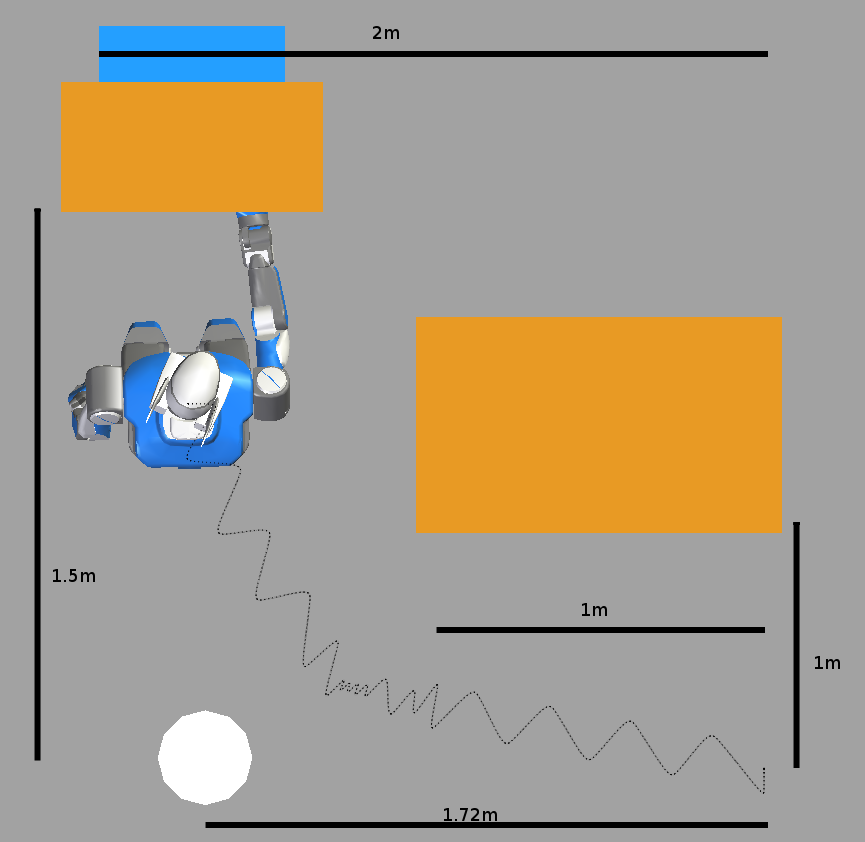
\includegraphics[width=.75\linewidth]{src/chap3-primitive-mouvement/dimensions.png}
    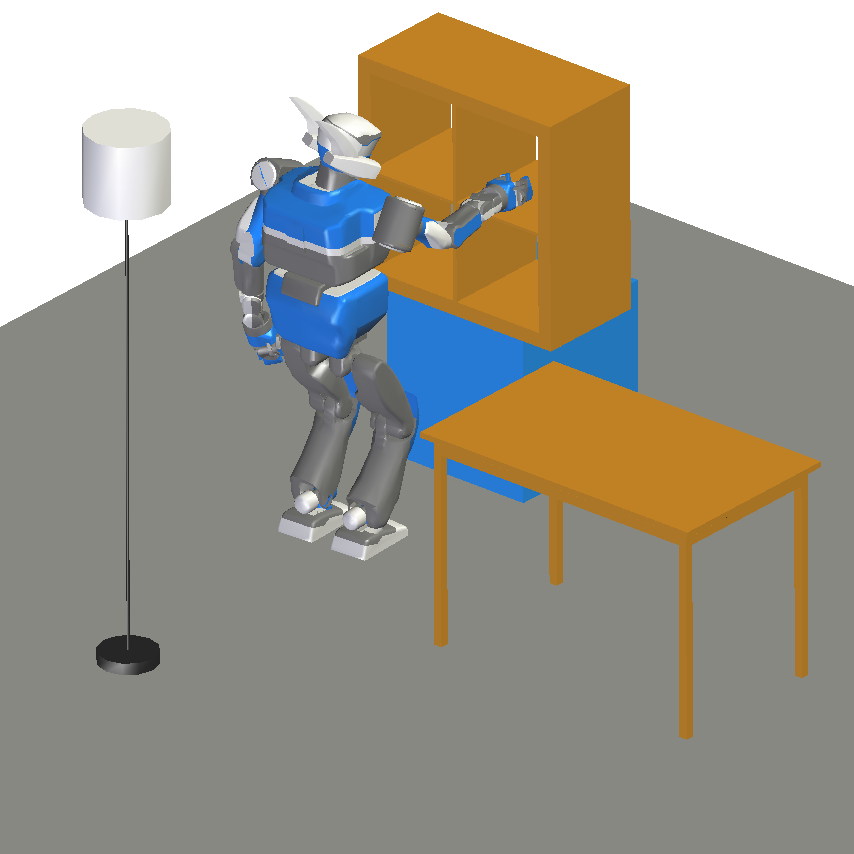
\includegraphics[width=.75\linewidth]{src/chap3-primitive-mouvement/trajectory-8.png}
  \end{center}
  \caption{Description de l'expérimentation: le robot part de la
    droite de l'image et progresse vers l'étagère située à gauche pour
    y déposer une balle. \label{fig:scenario_visu}}
\end{figure}



Le scénario proposé est le suivant: HRP-2\index{HRP-2} contourne un
obstacle, passe entre deux objets, et va poser une balle dans une
étagère. La longueur de la trajectoire de marche -- 2 mètres environ
-- et le nombre de pas génèrent une dérive suffisante pour qu'une
exécution de ce scénario échoue en boucle ouverte. En effet, passer
son bras dans une étagère est un mouvement contraint particulièrement
sensible à la position d'arrivée du robot. Une petite erreur dans le
positionnement du robot à la fin de la trajectoire engendrera une
grande erreur dans la position finale du poignet. La figure
\autoref{fig:scenario_visu} illustre le scénario.  L'objectif ici est
d'utiliser les caméras embarquées pour construire une carte de
l'environnement puis pour localiser le robot. La stratégie adoptée ici
n'est pas du SLAM -- Simultaneous Localization and Mapping
--\index{Simultaneous Localization and Mapping (SLAM)} dans la mesure
où les images permettant de construire la carte sont traitées hors
ligne. On réalise donc un premier mouvement sans correction afin
d'acquérir une séquence d'images permettant de construire la carte
puis on utilise cette carte pour localiser le robot durant les
expérimentations suivantes. La qualité du résultat est ensuite validée
en utilisant un système de capture de mouvement.


Durant les expériences, le module de localisation a fourni une
estimation de la position du robot à 16\hertz. Les images ont une
résolution de 320x240 pixels. L'ordinateur sur lequel fonctionne le
composant de localisation est un Intel\textregistered
Core\texttrademark\ 2 CPU T7200 @ 2.00GHz avec 2Gb.\ de RAM.


\subsection{Analyse de la précision du système de localisation}

La précision finale du système est illustrée par la
\autoref{fig:scenario_visu_precision}. On peut y observer une erreur à
la fin de la trajectoire d'environ 0.2 mètres en
translation. Plusieurs raisons peuvent expliquer ces mauvais
résultats:
\begin{enumerate}
\item Carte non métrique et absence de fermeture de boucle,
\item Passage dans des zones où la carte est peu dense ou dans des
  zones ne possédant que peu d'information visuelle,
\item Flexibilité du robot et/ou mauvaise identification de certains paramètres,
\end{enumerate}


Le premier point pouvant amener à une mauvaise estimation de la
localisation du robot est l'absence de fermeture de boucle. Les
techniques de localisation utilisant les informations visuelles
peuvent être divisées en deux catégories: odométrie
visuelle\index{odométrie visuelle} et localisation
``globale''. L'odométrie visuelle observe les changements entre deux
images aux temps $t_{n-1}$ et $t_n$ afin d'estimer la vitesse de la
caméra entre les deux images. Cette vitesse est ensuité intégrée pour
calculer le mouvement de la caméra. Le résultat de cette intégration
une dérive temporelle qui empêche toute tentative de localisation sur
le long terme en utilisant cette technique. Inversement, les
algorithmes utilisant une carte peuvent identifier les amères déjà
détectées auparavant et stabiliser le système. Une limite de ce
mouvement est qu'il n'est pas facile pour le système de reconnaître
des amères déjà identifiées. Il peut donc s'en suivre une dérive dans
l'estimation de la position du robot.


Le second problème concerne l'environnement en lui-même: à la fin du
mouvement, le robot se trouve face au meuble ce qui rend les images
captées par les caméras vide de toute amère permettant d'effectuer
correctement la localisation. Ce problème ne peut expliquer que
partiellement la mauvaise estimation dans la mesure où l'occlusion des
caméras n'intervient qu'à l'extrême fin du mouvement.


Le dernier point pouvant amener à une mauvaise estimation de l'erreur
est lié à la mauvaise modélisation de la chaîne cinématique du
robot. Une première erreur est liée à la présence, au niveau des
chevilles du robot, d'une flexibilité passive pouvant être modélisé
sous la forme de trois ressorts: deux autorisant un mouvement en
rotation et un troisième un déplacement en translation, c'est à dire
autorisant une compression de la cheville lors de la marche. Ce
dispositif a été conçu pour absorber les chocs et protéger le capteur
de force situé dans la cheville mais insère trois degrés de liberté
non modélisés et surtout non mesurables, car dépourvu
d'encodeur. Cette déformation au niveau de la cheville est donc
ignorée dans les calculs ce qui amène à un biais sur la position
relative du pied et de la tête du robot. Ce biais est d'autant plus
critique dans ce cas que c'est la position des points de contact que
l'on essaie de corriger. Une seconde source d'erreur est la
calibration de la position de la caméra dans le robot. Les
imprécisions de la conception du robot, du système de fixation des
caméras rendent nécessaire le calcul de la position relative de la
caméra par rapport au corps auquel il est fixé, dans notre cas la
tête. Un procédé de calibration des paramètres
extrinsèque\index{paramètres extrinsèques (d'une caméra)} a donc été
mis en place pour estimer ces paramètres. Ces derniers ont été validés
en reprojetant le modèle du robot dans l'image comme illustré par la
\autoref{fig:reprojection_modele_vision}.


\subsection{Résultats de la localisation utilisant la vision sur le robot humanoïde HRP-2}

L'ensemble de ces facteurs rend la réalisation d'un algorithme de
localisation embarqué sur HRP-2\index{HRP-2} délicat. Pour réaliser
une tâche de manipulation, une précision de l'ordre du centimètre est
souvent nécessaire. Or, les mauvaises performances du système de
localisation engendrent un bruit dans le positionnement du robot qui
peut rendre l'exécution de tâche précises délicate. Dans le scénario
choisit, la tâche peut être réalisée avec succès pour certains essais,
mais le taux d'échec restant très fort, cette méthode ne peut pas
constituer une boîte noire permettant de manière automatique de
réaliser un mouvement asservi. Une façon de résoudre le problème
serait de corriger la position du bras. En effet, entre la caméra et
le bras, la chaîne cinématique est bien identifiée. On voit donc ici
que l'approche consistant à avoir plusieurs systèmes de localisation
simultanément se justifie en pratique. Un composant de localisation
``global'' tel que celui utilisé ici permet de rendre la navigation
robuste sans toutefois être suffisant pour les tâches de
manipulation. Pour ces dernières, d'autres stratégies doivent être
envisagées comme la détection dans l'image de l'objet à attraper pour
asservir la position de la pince. On voit ici que plus qu'une
localisation parfaite sur le long terme, il est plus critique pour nos
scénarii d'avoir des algorithmes de localisation locaux assurant une
erreur minimale à la fin de la réalisation de la tâche. Les
algorithmes réalisant une localisation sur le long terme étant plutôt
destiné à alimenter les algorithmes de planification que les
algorithmes de contrôle nécessitant une haute précision sur la pose
estimée du robot.




\begin{figure}
  \begin{center}
    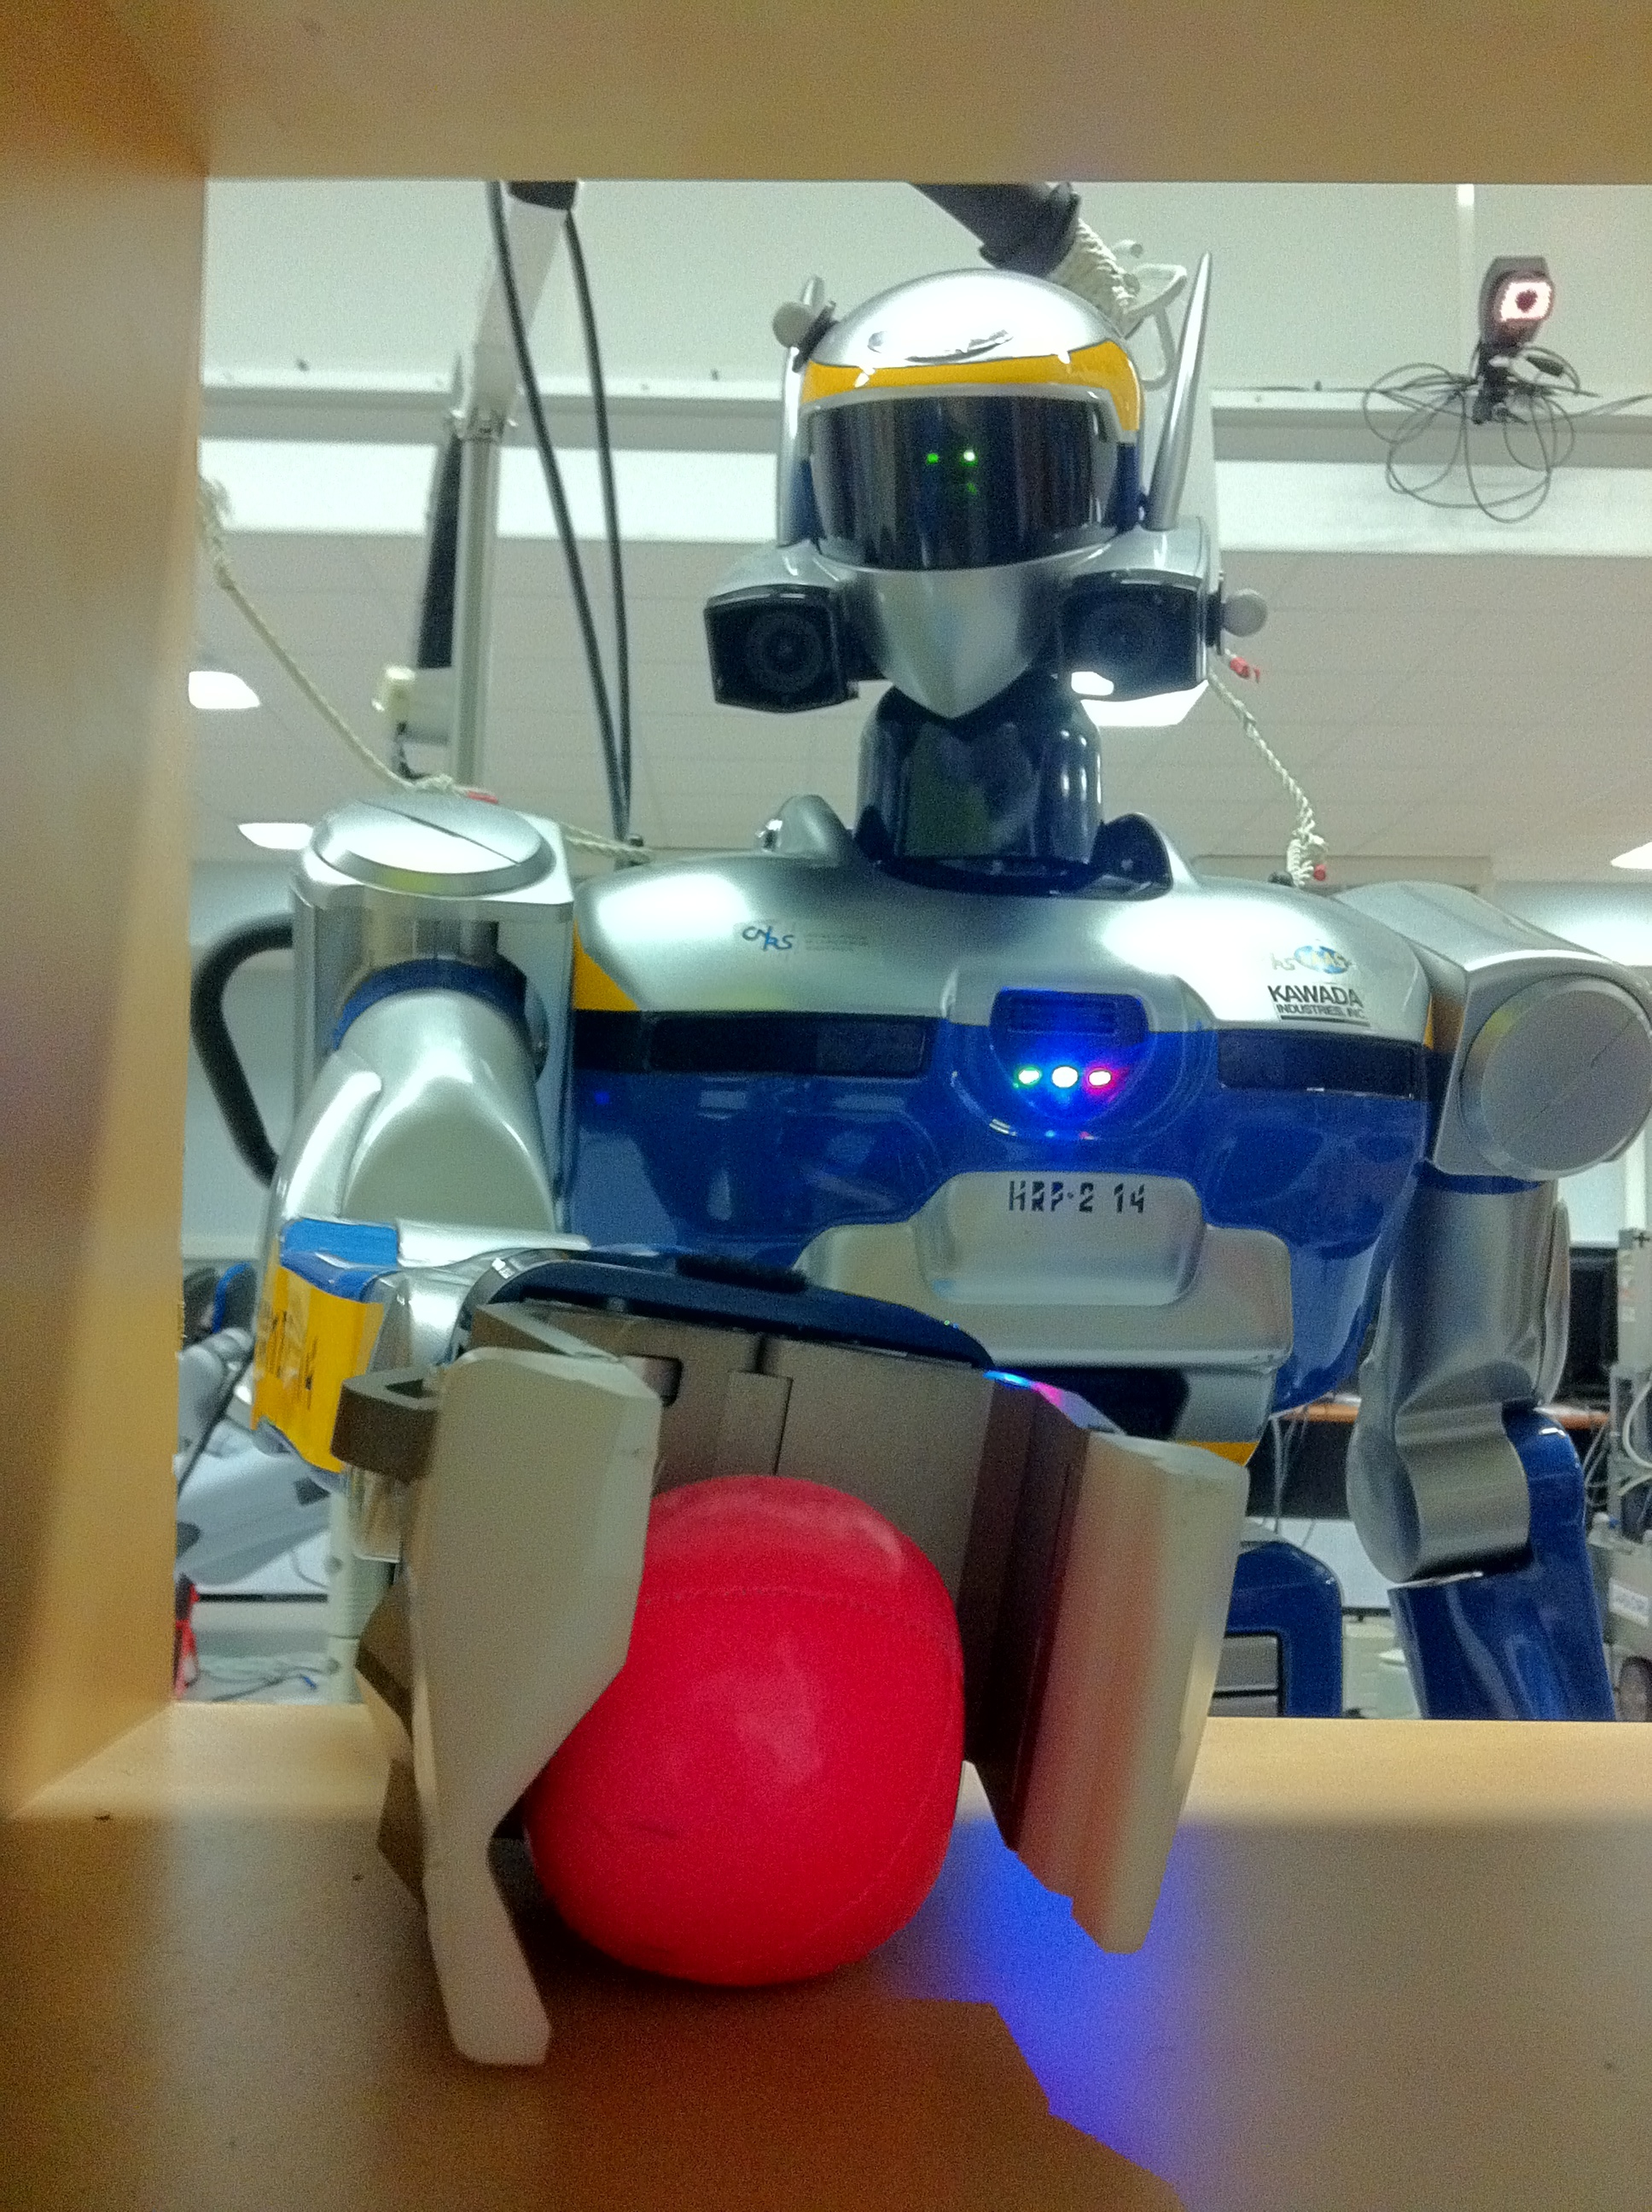
\includegraphics[width=.95\linewidth]{src/chap3-primitive-mouvement/demo1.jpg}
  \end{center}
  \caption{HRP-2 place une balle dans une étagère (I).}
\end{figure}

\begin{figure}
  \begin{center}
    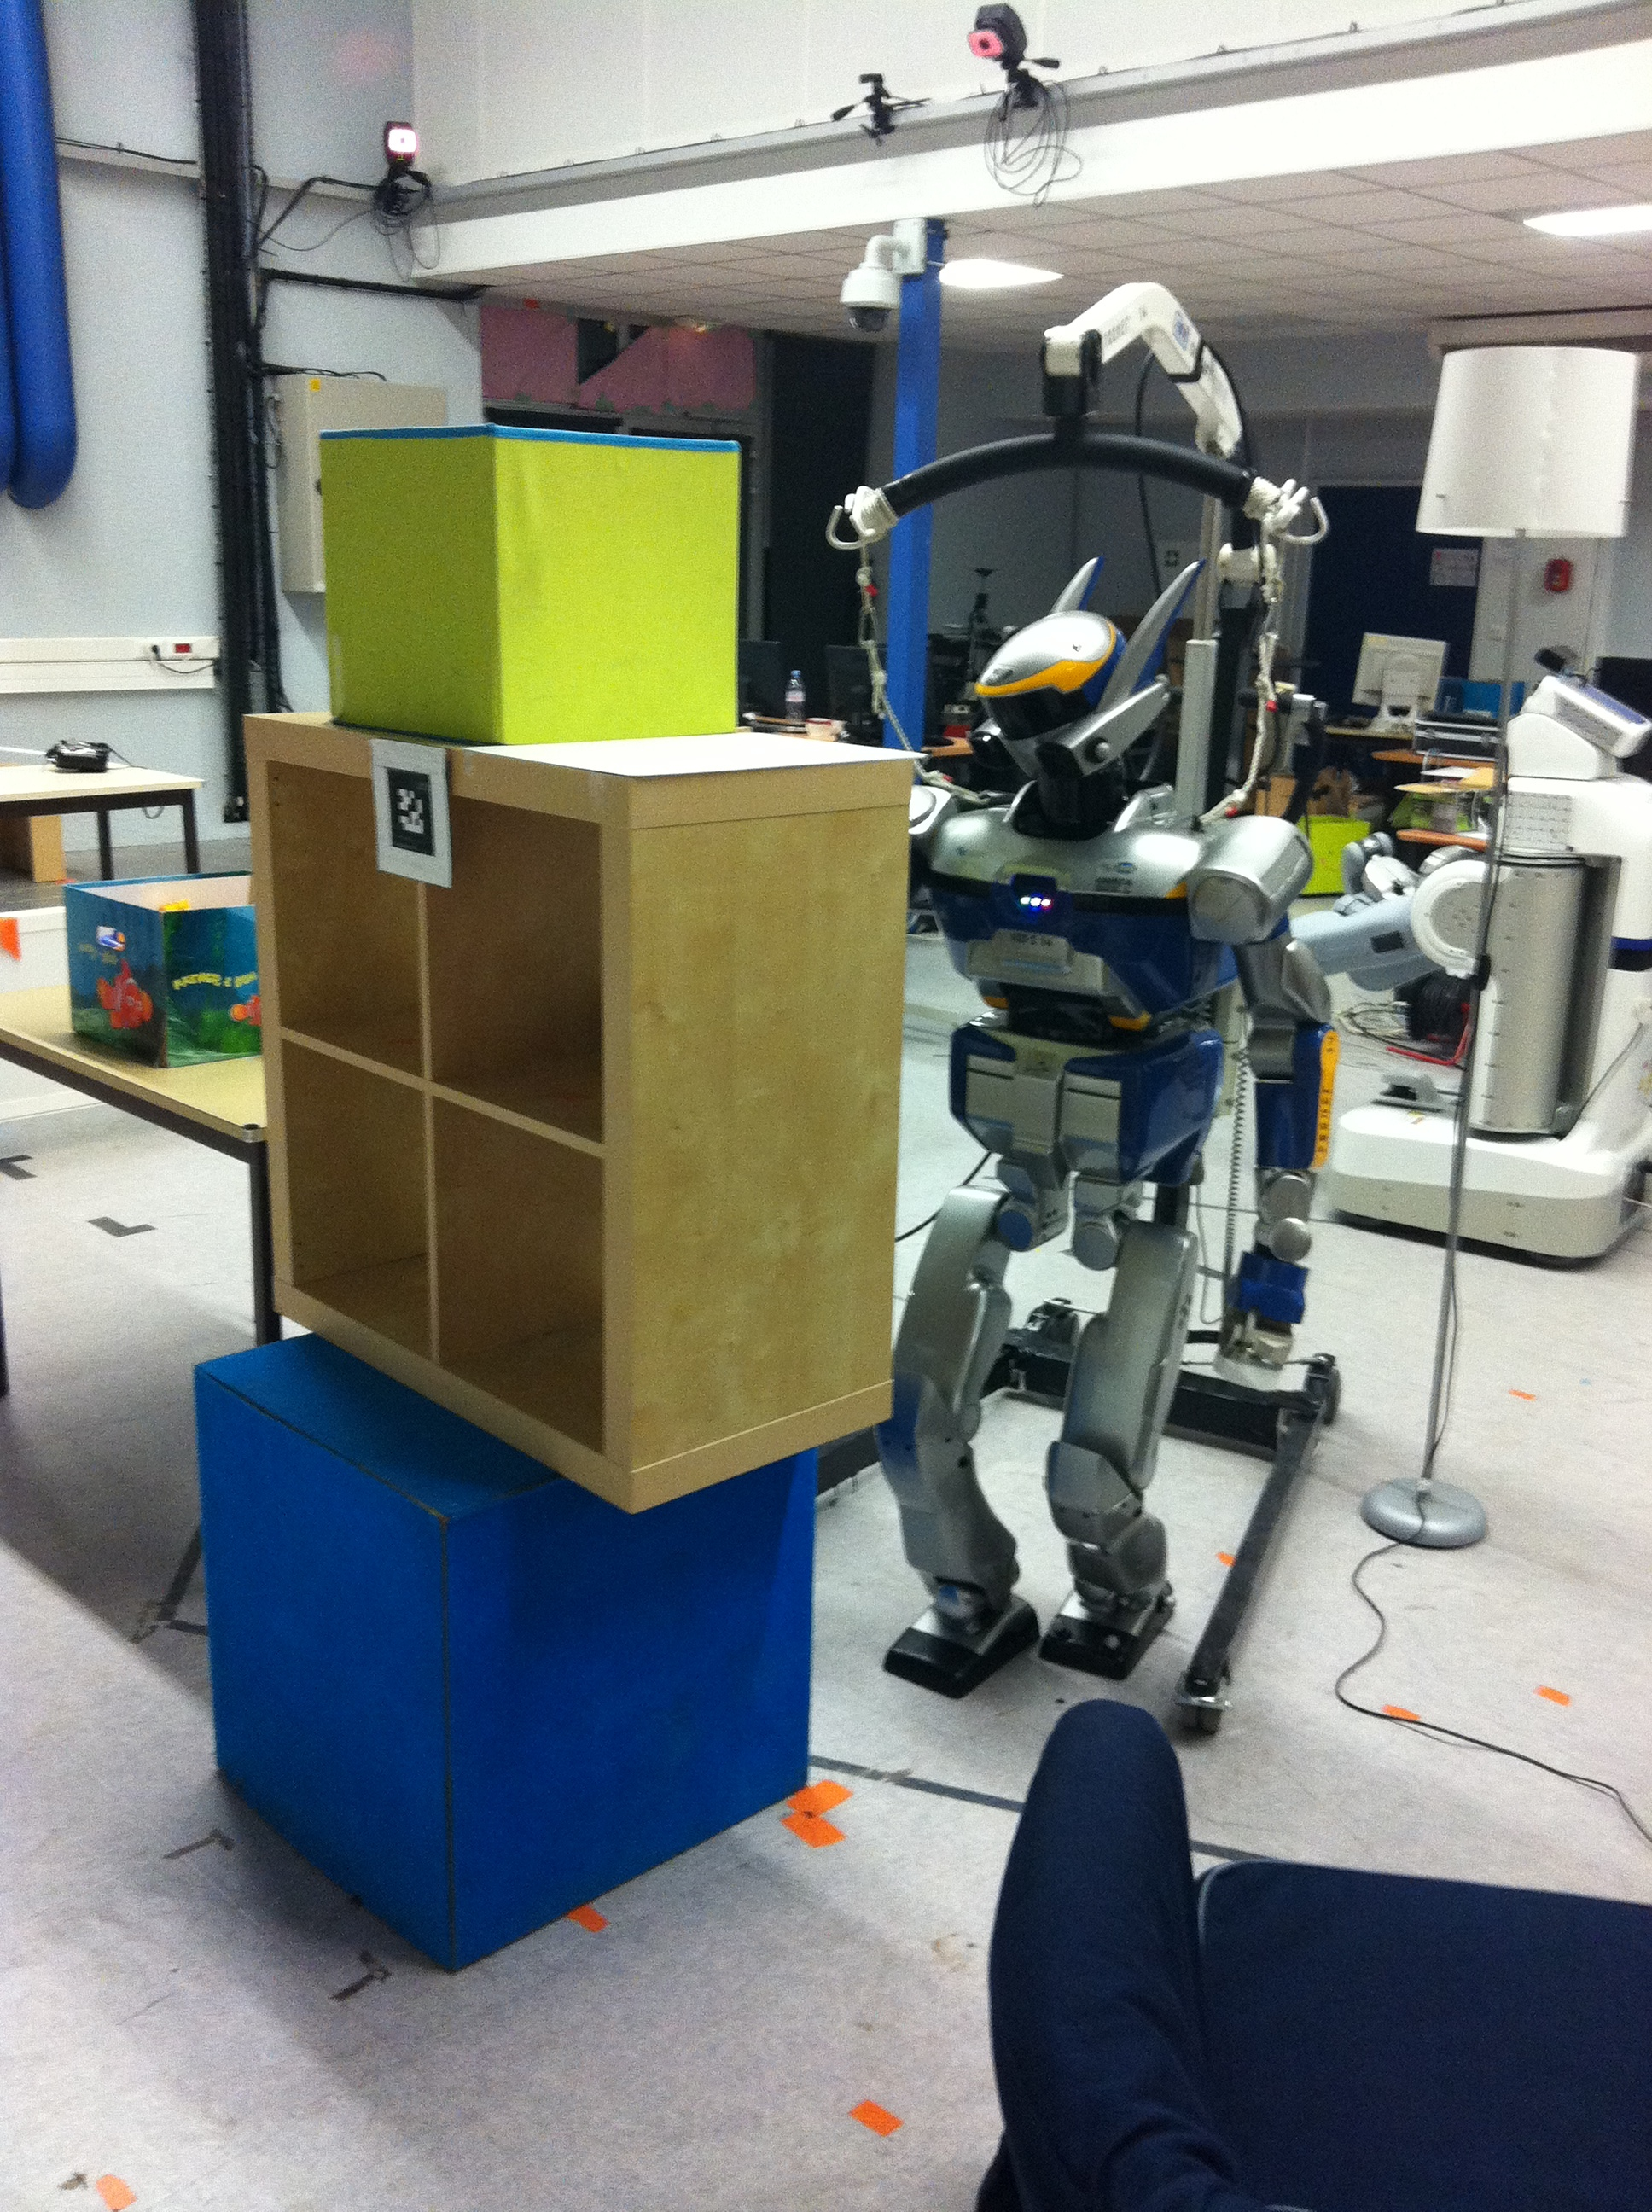
\includegraphics[width=.95\linewidth]{src/chap3-primitive-mouvement/demo2.jpg}
  \end{center}
  \caption{HRP-2 place une balle dans une étagère (II).}
\end{figure}


\begin{figure}
  \begin{center}
    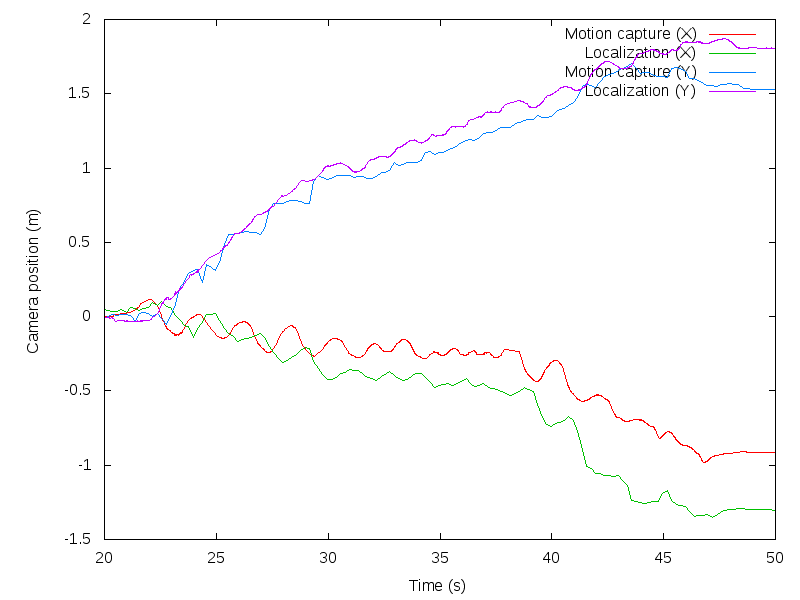
\includegraphics[width=.95\linewidth]{src/chap3-primitive-mouvement/mocap.png}
  \end{center}
  \caption{Précision de l'algorithme de SLAM par rapport au système de
    capture de mouvemement. \label{fig:scenario_visu_precision}}
\end{figure}

\begin{figure}
  \begin{center}
    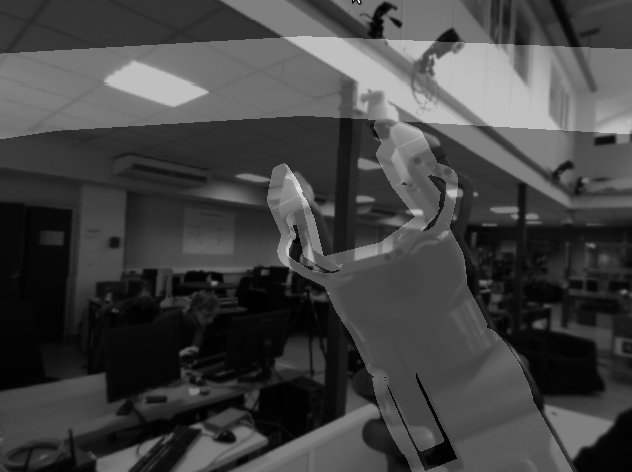
\includegraphics[width=.95\linewidth]{src/chap3-primitive-mouvement/calibextrinsic.jpg}
  \end{center}
  \caption{Reprojection du modèle du robot dans l'image captée par une
    caméra embarquée pour valider la calibration des paramètres de
    cette dernière. \label{fig:reprojection_modele_vision}}
\end{figure}


\section{Conclusion}

Pour continuer à explorer l'expression de plans de mouvement, il
faudrait donc intégrer de nouveaux algorithmes de localisation dédiés
à l'asservissement d'une tâche spécifique plutôt que d'envisager le
problème comme un bloc unitaire. La seconde partie des travaux reste
d'intégrer directement dans la phase de planification une étape de
planification des asservissements. L'idée est de planifier le
mouvement tel que le robot privilégiera le passage dans des zones où
la qualité de la localisation est maximale. En particulier, la
trajectoire de la tête sera calculée afin de laisser les amères
détectables le plus longtemps possible utilisables. Ce planificateur
pourra alors générer la partie asservissement du plan de mouvement
automatiquement. L'intégration de ces deux éléments reste des objectif
clé pour atteindre l'objectif de pouvoir asservir n'importe quel
mouvement sur un robot humanoïde de manière automatique.
